\documentclass{standalone}
\usepackage{tikz}
\usetikzlibrary{patterns, positioning}

\begin{document}
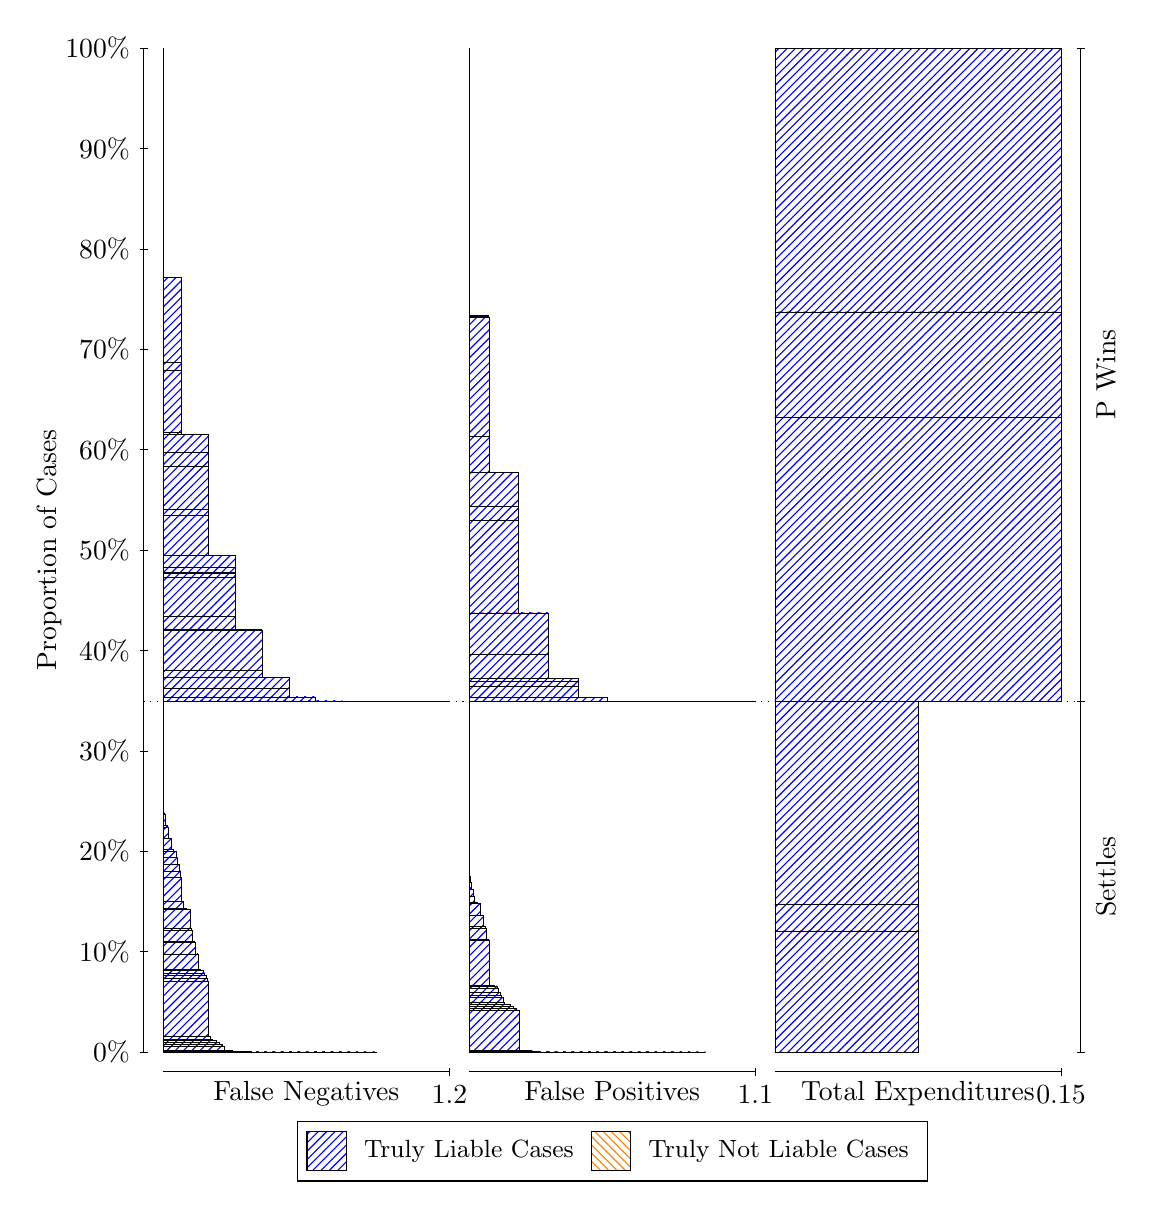
\begin{tikzpicture}
\draw[black, very thin] (1.5,1.75) -- (1.5,14.5);
\node[rotate=90, anchor=center] at (0.3, 8.125) {Proportion of Cases};
\draw[black, very thin] (1.45,1.75) -- (1.55,1.75);
\node[anchor=east] at (1.45, 1.75) {0\%};
\draw[black, very thin] (1.45,3.025) -- (1.55,3.025);
\node[anchor=east] at (1.45, 3.025) {10\%};
\draw[black, very thin] (1.45,4.3) -- (1.55,4.3);
\node[anchor=east] at (1.45, 4.3) {20\%};
\draw[black, very thin] (1.45,5.575) -- (1.55,5.575);
\node[anchor=east] at (1.45, 5.575) {30\%};
\draw[black, very thin] (1.45,6.85) -- (1.55,6.85);
\node[anchor=east] at (1.45, 6.85) {40\%};
\draw[black, very thin] (1.45,8.125) -- (1.55,8.125);
\node[anchor=east] at (1.45, 8.125) {50\%};
\draw[black, very thin] (1.45,9.4) -- (1.55,9.4);
\node[anchor=east] at (1.45, 9.4) {60\%};
\draw[black, very thin] (1.45,10.675) -- (1.55,10.675);
\node[anchor=east] at (1.45, 10.675) {70\%};
\draw[black, very thin] (1.45,11.95) -- (1.55,11.95);
\node[anchor=east] at (1.45, 11.95) {80\%};
\draw[black, very thin] (1.45,13.225) -- (1.55,13.225);
\node[anchor=east] at (1.45, 13.225) {90\%};
\draw[black, very thin] (1.45,14.5) -- (1.55,14.5);
\node[anchor=east] at (1.45, 14.5) {100\%};

\draw[black, very thin] (13.4,1.75) -- (13.4,14.5);
\draw[black, very thin] (13.35,1.75) -- (13.45,1.75);
\node[anchor=west] at (13.35, 1.75) {};
\draw[black, very thin] (13.35,6.2014) -- (13.45,6.2014);
\node[anchor=west] at (13.35, 6.2014) {};
\draw[black, very thin] (13.35,14.5) -- (13.45,14.5);
\node[anchor=west] at (13.35, 14.5) {};

\draw[black, very thin, pattern color=blue, pattern=north east lines] (1.75,1.75) rectangle (4.4654,1.75);
\draw[black, very thin, pattern color=blue, pattern=north east lines] (1.75,1.75) rectangle (4.3125,1.75);
\draw[black, very thin, pattern color=blue, pattern=north east lines] (1.75,1.75) rectangle (4.1595,1.75);
\draw[black, very thin, pattern color=blue, pattern=north east lines] (1.75,1.75) rectangle (4.1255,1.75);
\draw[black, very thin, pattern color=blue, pattern=north east lines] (1.75,1.75) rectangle (4.0065,1.75);
\draw[black, very thin, pattern color=blue, pattern=north east lines] (1.75,1.75) rectangle (3.9725,1.75);
\draw[black, very thin, pattern color=blue, pattern=north east lines] (1.75,1.75) rectangle (3.8535,1.75);
\draw[black, very thin, pattern color=blue, pattern=north east lines] (1.75,1.75) rectangle (3.8195,1.75);
\draw[black, very thin, pattern color=blue, pattern=north east lines] (1.75,1.75) rectangle (3.7855,1.75);
\draw[black, very thin, pattern color=blue, pattern=north east lines] (1.75,1.75) rectangle (3.7005,1.75);
\draw[black, very thin, pattern color=blue, pattern=north east lines] (1.75,1.75) rectangle (3.6665,1.75);
\draw[black, very thin, pattern color=blue, pattern=north east lines] (1.75,1.75) rectangle (3.6325,1.75);
\draw[black, very thin, pattern color=blue, pattern=north east lines] (1.75,1.75) rectangle (3.5475,1.75);
\draw[black, very thin, pattern color=blue, pattern=north east lines] (1.75,1.75) rectangle (3.5135,1.75);
\draw[black, very thin, pattern color=blue, pattern=north east lines] (1.75,1.75) rectangle (3.4796,1.75);
\draw[black, very thin, pattern color=blue, pattern=north east lines] (1.75,1.75) rectangle (3.4456,1.75);
\draw[black, very thin, pattern color=blue, pattern=north east lines] (1.75,1.75) rectangle (3.3946,1.75);
\draw[black, very thin, pattern color=blue, pattern=north east lines] (1.75,1.75) rectangle (3.3606,1.75);
\draw[black, very thin, pattern color=blue, pattern=north east lines] (1.75,1.75) rectangle (3.3266,1.75);
\draw[black, very thin, pattern color=blue, pattern=north east lines] (1.75,1.75) rectangle (3.2926,1.75);
\draw[black, very thin, pattern color=blue, pattern=north east lines] (1.75,1.75) rectangle (3.2416,1.75);
\draw[black, very thin, pattern color=blue, pattern=north east lines] (1.75,1.75) rectangle (3.2076,1.75);
\draw[black, very thin, pattern color=blue, pattern=north east lines] (1.75,1.75) rectangle (3.1736,1.75);
\draw[black, very thin, pattern color=blue, pattern=north east lines] (1.75,1.75) rectangle (3.1396,1.75);
\draw[black, very thin, pattern color=blue, pattern=north east lines] (1.75,1.75) rectangle (3.1056,1.75);
\draw[black, very thin, pattern color=blue, pattern=north east lines] (1.75,1.75) rectangle (3.0886,1.75);
\draw[black, very thin, pattern color=blue, pattern=north east lines] (1.75,1.75) rectangle (3.0546,1.75);
\draw[black, very thin, pattern color=blue, pattern=north east lines] (1.75,1.75) rectangle (3.0206,1.7501);
\draw[black, very thin, pattern color=blue, pattern=north east lines] (1.75,1.7501) rectangle (2.9866,1.7501);
\draw[black, very thin, pattern color=blue, pattern=north east lines] (1.75,1.7501) rectangle (2.9526,1.7502);
\draw[black, very thin, pattern color=blue, pattern=north east lines] (1.75,1.7502) rectangle (2.9356,1.7502);
\draw[black, very thin, pattern color=blue, pattern=north east lines] (1.75,1.7502) rectangle (2.9016,1.7503);
\draw[black, very thin, pattern color=blue, pattern=north east lines] (1.75,1.7503) rectangle (2.8676,1.7526);
\draw[black, very thin, pattern color=blue, pattern=north east lines] (1.75,1.7526) rectangle (2.8336,1.7533);
\draw[black, very thin, pattern color=blue, pattern=north east lines] (1.75,1.7533) rectangle (2.7996,1.7538);
\draw[black, very thin, pattern color=blue, pattern=north east lines] (1.75,1.7538) rectangle (2.7826,1.7539);
\draw[black, very thin, pattern color=blue, pattern=north east lines] (1.75,1.7539) rectangle (2.7656,1.7545);
\draw[black, very thin, pattern color=blue, pattern=north east lines] (1.75,1.7545) rectangle (2.7486,1.7546);
\draw[black, very thin, pattern color=blue, pattern=north east lines] (1.75,1.7546) rectangle (2.7146,1.7547);
\draw[black, very thin, pattern color=blue, pattern=north east lines] (1.75,1.7547) rectangle (2.6806,1.7595);
\draw[black, very thin, pattern color=blue, pattern=north east lines] (1.75,1.7595) rectangle (2.6466,1.7615);
\draw[black, very thin, pattern color=blue, pattern=north east lines] (1.75,1.7615) rectangle (2.6296,1.7656);
\draw[black, very thin, pattern color=blue, pattern=north east lines] (1.75,1.7656) rectangle (2.6127,1.7675);
\draw[black, very thin, pattern color=blue, pattern=north east lines] (1.75,1.7675) rectangle (2.5957,1.7697);
\draw[black, very thin, pattern color=blue, pattern=north east lines] (1.75,1.7697) rectangle (2.5617,1.7727);
\draw[black, very thin, pattern color=blue, pattern=north east lines] (1.75,1.7727) rectangle (2.5277,1.8211);
\draw[black, very thin, pattern color=blue, pattern=north east lines] (1.75,1.8211) rectangle (2.4937,1.8445);
\draw[black, very thin, pattern color=blue, pattern=north east lines] (1.75,1.8445) rectangle (2.4767,1.8506);
\draw[black, very thin, pattern color=blue, pattern=north east lines] (1.75,1.8506) rectangle (2.4597,1.8723);
\draw[black, very thin, pattern color=blue, pattern=north east lines] (1.75,1.8723) rectangle (2.4427,1.8757);
\draw[black, very thin, pattern color=blue, pattern=north east lines] (1.75,1.8757) rectangle (2.4257,1.9014);
\draw[black, very thin, pattern color=blue, pattern=north east lines] (1.75,1.9014) rectangle (2.4087,1.9032);
\draw[black, very thin, pattern color=blue, pattern=north east lines] (1.75,1.9032) rectangle (2.3747,1.9051);
\draw[black, very thin, pattern color=blue, pattern=north east lines] (1.75,1.9051) rectangle (2.3407,1.9534);
\draw[black, very thin, pattern color=blue, pattern=north east lines] (1.75,1.9534) rectangle (2.3237,2.6531);
\draw[black, very thin, pattern color=blue, pattern=north east lines] (1.75,2.6531) rectangle (2.3067,2.6851);
\draw[black, very thin, pattern color=blue, pattern=north east lines] (1.75,2.6851) rectangle (2.2897,2.7212);
\draw[black, very thin, pattern color=blue, pattern=north east lines] (1.75,2.7212) rectangle (2.2727,2.7537);
\draw[black, very thin, pattern color=blue, pattern=north east lines] (1.75,2.7537) rectangle (2.2557,2.7841);
\draw[black, very thin, pattern color=blue, pattern=north east lines] (1.75,2.7841) rectangle (2.2217,2.8033);
\draw[black, very thin, pattern color=blue, pattern=north east lines] (1.75,2.8033) rectangle (2.1877,2.9963);
\draw[black, very thin, pattern color=blue, pattern=north east lines] (1.75,2.9963) rectangle (2.1537,3.1377);
\draw[black, very thin, pattern color=blue, pattern=north east lines] (1.75,3.1377) rectangle (2.1367,3.1591);
\draw[black, very thin, pattern color=blue, pattern=north east lines] (1.75,3.1591) rectangle (2.1197,3.2977);
\draw[black, very thin, pattern color=blue, pattern=north east lines] (1.75,3.2977) rectangle (2.1027,3.3166);
\draw[black, very thin, pattern color=blue, pattern=north east lines] (1.75,3.3166) rectangle (2.0857,3.5604);
\draw[black, very thin, pattern color=blue, pattern=north east lines] (1.75,3.5604) rectangle (2.0687,3.5652);
\draw[black, very thin, pattern color=blue, pattern=north east lines] (1.75,3.5652) rectangle (2.0347,3.5699);
\draw[black, very thin, pattern color=blue, pattern=north east lines] (1.75,3.5699) rectangle (2.0007,3.6631);
\draw[black, very thin, pattern color=blue, pattern=north east lines] (1.75,3.6631) rectangle (1.9837,3.9698);
\draw[black, very thin, pattern color=blue, pattern=north east lines] (1.75,3.9698) rectangle (1.9667,4.05);
\draw[black, very thin, pattern color=blue, pattern=north east lines] (1.75,4.05) rectangle (1.9497,4.1301);
\draw[black, very thin, pattern color=blue, pattern=north east lines] (1.75,4.1301) rectangle (1.9327,4.2245);
\draw[black, very thin, pattern color=blue, pattern=north east lines] (1.75,4.2245) rectangle (1.9157,4.2995);
\draw[black, very thin, pattern color=blue, pattern=north east lines] (1.75,4.2995) rectangle (1.8817,4.3186);
\draw[black, very thin, pattern color=blue, pattern=north east lines] (1.75,4.3186) rectangle (1.8477,4.4667);
\draw[black, very thin, pattern color=blue, pattern=north east lines] (1.75,4.4667) rectangle (1.8137,4.6053);
\draw[black, very thin, pattern color=blue, pattern=north east lines] (1.75,4.6053) rectangle (1.7967,4.6242);
\draw[black, very thin, pattern color=blue, pattern=north east lines] (1.75,4.6242) rectangle (1.7797,4.7673);
\draw[black, very thin, pattern color=blue, pattern=north east lines] (1.75,4.7673) rectangle (1.7627,4.786);
\draw[black, very thin, pattern color=orange, pattern=north west lines] (1.75,4.786) rectangle (1.75,4.786);
\draw[black, very thin, pattern color=blue, pattern=north east lines] (1.75,4.786) rectangle (1.75,6.2014);
\draw[black, very thin, pattern color=blue, pattern=north east lines] (1.75,6.2014) rectangle (5.3833,6.2014);
\draw[black, very thin, pattern color=blue, pattern=north east lines] (1.75,6.2014) rectangle (5.0434,6.2014);
\draw[black, very thin, pattern color=blue, pattern=north east lines] (1.75,6.2014) rectangle (4.7034,6.2014);
\draw[black, very thin, pattern color=blue, pattern=north east lines] (1.75,6.2014) rectangle (4.7034,6.2014);
\draw[black, very thin, pattern color=blue, pattern=north east lines] (1.75,6.2014) rectangle (4.6992,6.2014);
\draw[black, very thin, pattern color=blue, pattern=north east lines] (1.75,6.2014) rectangle (4.3635,6.2016);
\draw[black, very thin, pattern color=blue, pattern=north east lines] (1.75,6.2016) rectangle (4.3635,6.2019);
\draw[black, very thin, pattern color=blue, pattern=north east lines] (1.75,6.2019) rectangle (4.3592,6.2019);
\draw[black, very thin, pattern color=blue, pattern=north east lines] (1.75,6.2019) rectangle (4.3592,6.2019);
\draw[black, very thin, pattern color=blue, pattern=north east lines] (1.75,6.2019) rectangle (4.0235,6.2082);
\draw[black, very thin, pattern color=blue, pattern=north east lines] (1.75,6.2082) rectangle (4.0192,6.2082);
\draw[black, very thin, pattern color=blue, pattern=north east lines] (1.75,6.2082) rectangle (3.6835,6.2583);
\draw[black, very thin, pattern color=blue, pattern=north east lines] (1.75,6.2583) rectangle (3.6793,6.2583);
\draw[black, very thin, pattern color=blue, pattern=north east lines] (1.75,6.2583) rectangle (3.3436,6.3628);
\draw[black, very thin, pattern color=blue, pattern=north east lines] (1.75,6.3628) rectangle (3.3436,6.5026);
\draw[black, very thin, pattern color=blue, pattern=north east lines] (1.75,6.5026) rectangle (3.3393,6.5026);
\draw[black, very thin, pattern color=blue, pattern=north east lines] (1.75,6.5026) rectangle (3.3393,6.5027);
\draw[black, very thin, pattern color=blue, pattern=north east lines] (1.75,6.5027) rectangle (3.0036,6.5985);
\draw[black, very thin, pattern color=blue, pattern=north east lines] (1.75,6.5985) rectangle (3.0036,7.1084);
\draw[black, very thin, pattern color=blue, pattern=north east lines] (1.75,7.1084) rectangle (2.9994,7.109);
\draw[black, very thin, pattern color=blue, pattern=north east lines] (1.75,7.109) rectangle (2.9994,7.1167);
\draw[black, very thin, pattern color=blue, pattern=north east lines] (1.75,7.1167) rectangle (2.9994,7.1209);
\draw[black, very thin, pattern color=blue, pattern=north east lines] (1.75,7.1209) rectangle (2.6636,7.2896);
\draw[black, very thin, pattern color=blue, pattern=north east lines] (1.75,7.2896) rectangle (2.6636,7.7803);
\draw[black, very thin, pattern color=blue, pattern=north east lines] (1.75,7.7803) rectangle (2.6636,7.8307);
\draw[black, very thin, pattern color=blue, pattern=north east lines] (1.75,7.8307) rectangle (2.6594,7.8401);
\draw[black, very thin, pattern color=blue, pattern=north east lines] (1.75,7.8401) rectangle (2.6594,7.9057);
\draw[black, very thin, pattern color=blue, pattern=north east lines] (1.75,7.9057) rectangle (2.6594,8.0603);
\draw[black, very thin, pattern color=blue, pattern=north east lines] (1.75,8.0603) rectangle (2.3237,8.5627);
\draw[black, very thin, pattern color=blue, pattern=north east lines] (1.75,8.5627) rectangle (2.3194,8.6413);
\draw[black, very thin, pattern color=blue, pattern=north east lines] (1.75,8.6413) rectangle (2.3194,9.1927);
\draw[black, very thin, pattern color=blue, pattern=north east lines] (1.75,9.1927) rectangle (2.3194,9.369);
\draw[black, very thin, pattern color=blue, pattern=north east lines] (1.75,9.369) rectangle (2.3194,9.5957);
\draw[black, very thin, pattern color=blue, pattern=north east lines] (1.75,9.5957) rectangle (1.9837,9.5959);
\draw[black, very thin, pattern color=blue, pattern=north east lines] (1.75,9.5959) rectangle (1.9837,9.6178);
\draw[black, very thin, pattern color=blue, pattern=north east lines] (1.75,9.6178) rectangle (1.9837,9.6179);
\draw[black, very thin, pattern color=blue, pattern=north east lines] (1.75,9.6179) rectangle (1.9795,10.405);
\draw[black, very thin, pattern color=blue, pattern=north east lines] (1.75,10.405) rectangle (1.9795,10.508);
\draw[black, very thin, pattern color=blue, pattern=north east lines] (1.75,10.508) rectangle (1.9795,11.589);
\draw[black, very thin, pattern color=orange, pattern=north west lines] (1.75,11.589) rectangle (1.75,11.589);
\draw[black, very thin, pattern color=blue, pattern=north east lines] (1.75,11.589) rectangle (1.75,14.5);
\draw[black, very thin, pattern color=orange, pattern=north west lines] (5.6333,1.75) rectangle (8.6329,1.75);
\draw[black, very thin, pattern color=blue, pattern=north east lines] (5.6333,1.75) rectangle (8.6329,1.75);
\draw[black, very thin, pattern color=orange, pattern=north west lines] (5.6333,1.75) rectangle (8.464,1.75);
\draw[black, very thin, pattern color=blue, pattern=north east lines] (5.6333,1.75) rectangle (8.464,1.75);
\draw[black, very thin, pattern color=orange, pattern=north west lines] (5.6333,1.75) rectangle (8.295,1.75);
\draw[black, very thin, pattern color=blue, pattern=north east lines] (5.6333,1.75) rectangle (8.295,1.75);
\draw[black, very thin, pattern color=blue, pattern=north east lines] (5.6333,1.75) rectangle (8.2574,1.75);
\draw[black, very thin, pattern color=orange, pattern=north west lines] (5.6333,1.75) rectangle (8.126,1.75);
\draw[black, very thin, pattern color=blue, pattern=north east lines] (5.6333,1.75) rectangle (8.126,1.75);
\draw[black, very thin, pattern color=blue, pattern=north east lines] (5.6333,1.75) rectangle (8.0884,1.75);
\draw[black, very thin, pattern color=orange, pattern=north west lines] (5.6333,1.75) rectangle (7.957,1.75);
\draw[black, very thin, pattern color=blue, pattern=north east lines] (5.6333,1.75) rectangle (7.957,1.75);
\draw[black, very thin, pattern color=blue, pattern=north east lines] (5.6333,1.75) rectangle (7.9194,1.75);
\draw[black, very thin, pattern color=blue, pattern=north east lines] (5.6333,1.75) rectangle (7.8819,1.75);
\draw[black, very thin, pattern color=orange, pattern=north west lines] (5.6333,1.75) rectangle (7.788,1.75);
\draw[black, very thin, pattern color=blue, pattern=north east lines] (5.6333,1.75) rectangle (7.788,1.75);
\draw[black, very thin, pattern color=blue, pattern=north east lines] (5.6333,1.75) rectangle (7.7504,1.75);
\draw[black, very thin, pattern color=blue, pattern=north east lines] (5.6333,1.75) rectangle (7.7129,1.75);
\draw[black, very thin, pattern color=orange, pattern=north west lines] (5.6333,1.75) rectangle (7.619,1.75);
\draw[black, very thin, pattern color=blue, pattern=north east lines] (5.6333,1.75) rectangle (7.619,1.75);
\draw[black, very thin, pattern color=blue, pattern=north east lines] (5.6333,1.75) rectangle (7.5814,1.75);
\draw[black, very thin, pattern color=blue, pattern=north east lines] (5.6333,1.75) rectangle (7.5439,1.75);
\draw[black, very thin, pattern color=blue, pattern=north east lines] (5.6333,1.75) rectangle (7.5063,1.75);
\draw[black, very thin, pattern color=orange, pattern=north west lines] (5.6333,1.75) rectangle (7.45,1.75);
\draw[black, very thin, pattern color=blue, pattern=north east lines] (5.6333,1.75) rectangle (7.45,1.75);
\draw[black, very thin, pattern color=blue, pattern=north east lines] (5.6333,1.75) rectangle (7.4124,1.75);
\draw[black, very thin, pattern color=blue, pattern=north east lines] (5.6333,1.75) rectangle (7.3749,1.75);
\draw[black, very thin, pattern color=blue, pattern=north east lines] (5.6333,1.75) rectangle (7.3373,1.75);
\draw[black, very thin, pattern color=orange, pattern=north west lines] (5.6333,1.75) rectangle (7.281,1.75);
\draw[black, very thin, pattern color=blue, pattern=north east lines] (5.6333,1.75) rectangle (7.281,1.75);
\draw[black, very thin, pattern color=blue, pattern=north east lines] (5.6333,1.75) rectangle (7.2435,1.75);
\draw[black, very thin, pattern color=blue, pattern=north east lines] (5.6333,1.75) rectangle (7.2059,1.75);
\draw[black, very thin, pattern color=blue, pattern=north east lines] (5.6333,1.75) rectangle (7.1683,1.75);
\draw[black, very thin, pattern color=blue, pattern=north east lines] (5.6333,1.75) rectangle (7.1308,1.75);
\draw[black, very thin, pattern color=orange, pattern=north west lines] (5.6333,1.75) rectangle (7.112,1.75);
\draw[black, very thin, pattern color=blue, pattern=north east lines] (5.6333,1.75) rectangle (7.112,1.75);
\draw[black, very thin, pattern color=blue, pattern=north east lines] (5.6333,1.75) rectangle (7.0745,1.75);
\draw[black, very thin, pattern color=blue, pattern=north east lines] (5.6333,1.75) rectangle (7.0369,1.75);
\draw[black, very thin, pattern color=blue, pattern=north east lines] (5.6333,1.75) rectangle (6.9994,1.75);
\draw[black, very thin, pattern color=blue, pattern=north east lines] (5.6333,1.75) rectangle (6.9618,1.75);
\draw[black, very thin, pattern color=orange, pattern=north west lines] (5.6333,1.75) rectangle (6.943,1.75);
\draw[black, very thin, pattern color=blue, pattern=north east lines] (5.6333,1.75) rectangle (6.943,1.75);
\draw[black, very thin, pattern color=blue, pattern=north east lines] (5.6333,1.75) rectangle (6.9055,1.75);
\draw[black, very thin, pattern color=blue, pattern=north east lines] (5.6333,1.75) rectangle (6.8679,1.75);
\draw[black, very thin, pattern color=blue, pattern=north east lines] (5.6333,1.75) rectangle (6.8304,1.75);
\draw[black, very thin, pattern color=blue, pattern=north east lines] (5.6333,1.75) rectangle (6.7928,1.75);
\draw[black, very thin, pattern color=orange, pattern=north west lines] (5.6333,1.75) rectangle (6.774,1.75);
\draw[black, very thin, pattern color=blue, pattern=north east lines] (5.6333,1.75) rectangle (6.774,1.7501);
\draw[black, very thin, pattern color=blue, pattern=north east lines] (5.6333,1.7501) rectangle (6.7553,1.7501);
\draw[black, very thin, pattern color=blue, pattern=north east lines] (5.6333,1.7501) rectangle (6.7365,1.7501);
\draw[black, very thin, pattern color=blue, pattern=north east lines] (5.6333,1.7501) rectangle (6.6989,1.7501);
\draw[black, very thin, pattern color=blue, pattern=north east lines] (5.6333,1.7501) rectangle (6.6614,1.7501);
\draw[black, very thin, pattern color=blue, pattern=north east lines] (5.6333,1.7501) rectangle (6.6238,1.7502);
\draw[black, very thin, pattern color=orange, pattern=north west lines] (5.6333,1.7502) rectangle (6.605,1.7502);
\draw[black, very thin, pattern color=blue, pattern=north east lines] (5.6333,1.7502) rectangle (6.605,1.7515);
\draw[black, very thin, pattern color=blue, pattern=north east lines] (5.6333,1.7515) rectangle (6.5863,1.7516);
\draw[black, very thin, pattern color=blue, pattern=north east lines] (5.6333,1.7516) rectangle (6.5675,1.7522);
\draw[black, very thin, pattern color=blue, pattern=north east lines] (5.6333,1.7522) rectangle (6.5299,1.7527);
\draw[black, very thin, pattern color=blue, pattern=north east lines] (5.6333,1.7527) rectangle (6.4924,1.7528);
\draw[black, very thin, pattern color=blue, pattern=north east lines] (5.6333,1.7528) rectangle (6.4548,1.7546);
\draw[black, very thin, pattern color=orange, pattern=north west lines] (5.6333,1.7546) rectangle (6.436,1.7546);
\draw[black, very thin, pattern color=blue, pattern=north east lines] (5.6333,1.7546) rectangle (6.436,1.7646);
\draw[black, very thin, pattern color=blue, pattern=north east lines] (5.6333,1.7646) rectangle (6.4173,1.7665);
\draw[black, very thin, pattern color=blue, pattern=north east lines] (5.6333,1.7665) rectangle (6.3985,1.7689);
\draw[black, very thin, pattern color=blue, pattern=north east lines] (5.6333,1.7689) rectangle (6.3797,1.7712);
\draw[black, very thin, pattern color=blue, pattern=north east lines] (5.6333,1.7712) rectangle (6.3609,1.7732);
\draw[black, very thin, pattern color=blue, pattern=north east lines] (5.6333,1.7732) rectangle (6.3234,1.7733);
\draw[black, very thin, pattern color=blue, pattern=north east lines] (5.6333,1.7733) rectangle (6.2858,1.7734);
\draw[black, very thin, pattern color=orange, pattern=north west lines] (5.6333,1.7734) rectangle (6.2671,1.7734);
\draw[black, very thin, pattern color=blue, pattern=north east lines] (5.6333,1.7734) rectangle (6.2671,2.277);
\draw[black, very thin, pattern color=blue, pattern=north east lines] (5.6333,2.277) rectangle (6.2483,2.2799);
\draw[black, very thin, pattern color=blue, pattern=north east lines] (5.6333,2.2799) rectangle (6.2295,2.3068);
\draw[black, very thin, pattern color=blue, pattern=north east lines] (5.6333,2.3068) rectangle (6.2107,2.3097);
\draw[black, very thin, pattern color=blue, pattern=north east lines] (5.6333,2.3097) rectangle (6.1919,2.3317);
\draw[black, very thin, pattern color=blue, pattern=north east lines] (5.6333,2.3317) rectangle (6.1544,2.3523);
\draw[black, very thin, pattern color=blue, pattern=north east lines] (5.6333,2.3523) rectangle (6.1168,2.3553);
\draw[black, very thin, pattern color=blue, pattern=north east lines] (5.6333,2.3553) rectangle (6.0793,2.385);
\draw[black, very thin, pattern color=blue, pattern=north east lines] (5.6333,2.385) rectangle (6.0605,2.4404);
\draw[black, very thin, pattern color=blue, pattern=north east lines] (5.6333,2.4404) rectangle (6.0417,2.4718);
\draw[black, very thin, pattern color=blue, pattern=north east lines] (5.6333,2.4718) rectangle (6.023,2.5042);
\draw[black, very thin, pattern color=blue, pattern=north east lines] (5.6333,2.5042) rectangle (6.0042,2.5578);
\draw[black, very thin, pattern color=blue, pattern=north east lines] (5.6333,2.5578) rectangle (5.9854,2.5903);
\draw[black, very thin, pattern color=blue, pattern=north east lines] (5.6333,2.5903) rectangle (5.9478,2.5922);
\draw[black, very thin, pattern color=blue, pattern=north east lines] (5.6333,2.5922) rectangle (5.9103,2.5941);
\draw[black, very thin, pattern color=blue, pattern=north east lines] (5.6333,2.5941) rectangle (5.8915,3.1654);
\draw[black, very thin, pattern color=blue, pattern=north east lines] (5.6333,3.1654) rectangle (5.8727,3.184);
\draw[black, very thin, pattern color=blue, pattern=north east lines] (5.6333,3.184) rectangle (5.854,3.3272);
\draw[black, very thin, pattern color=blue, pattern=north east lines] (5.6333,3.3272) rectangle (5.8352,3.3461);
\draw[black, very thin, pattern color=blue, pattern=north east lines] (5.6333,3.3461) rectangle (5.8164,3.4847);
\draw[black, very thin, pattern color=blue, pattern=north east lines] (5.6333,3.4847) rectangle (5.7789,3.6328);
\draw[black, very thin, pattern color=blue, pattern=north east lines] (5.6333,3.6328) rectangle (5.7413,3.6519);
\draw[black, very thin, pattern color=blue, pattern=north east lines] (5.6333,3.6519) rectangle (5.7037,3.7269);
\draw[black, very thin, pattern color=blue, pattern=north east lines] (5.6333,3.7269) rectangle (5.685,3.8213);
\draw[black, very thin, pattern color=blue, pattern=north east lines] (5.6333,3.8213) rectangle (5.6662,3.9014);
\draw[black, very thin, pattern color=blue, pattern=north east lines] (5.6333,3.9014) rectangle (5.6474,3.9816);
\draw[black, very thin, pattern color=blue, pattern=north east lines] (5.6333,3.9816) rectangle (5.6333,6.2014);
\draw[black, very thin, pattern color=orange, pattern=north west lines] (5.6333,6.2014) rectangle (9.2667,6.2014);
\draw[black, very thin, pattern color=blue, pattern=north east lines] (5.6333,6.2014) rectangle (9.2667,6.2014);
\draw[black, very thin, pattern color=orange, pattern=north west lines] (5.6333,6.2014) rectangle (8.8911,6.2014);
\draw[black, very thin, pattern color=blue, pattern=north east lines] (5.6333,6.2014) rectangle (8.8911,6.2014);
\draw[black, very thin, pattern color=orange, pattern=north west lines] (5.6333,6.2014) rectangle (8.5156,6.2014);
\draw[black, very thin, pattern color=blue, pattern=north east lines] (5.6333,6.2014) rectangle (8.5156,6.2014);
\draw[black, very thin, pattern color=blue, pattern=north east lines] (5.6333,6.2014) rectangle (8.5156,6.2014);
\draw[black, very thin, pattern color=blue, pattern=north east lines] (5.6333,6.2014) rectangle (8.1401,6.2016);
\draw[black, very thin, pattern color=orange, pattern=north west lines] (5.6333,6.2016) rectangle (8.1401,6.2016);
\draw[black, very thin, pattern color=blue, pattern=north east lines] (5.6333,6.2016) rectangle (8.1401,6.2018);
\draw[black, very thin, pattern color=orange, pattern=north west lines] (5.6333,6.2018) rectangle (7.7645,6.2018);
\draw[black, very thin, pattern color=blue, pattern=north east lines] (5.6333,6.2018) rectangle (7.7645,6.2072);
\draw[black, very thin, pattern color=orange, pattern=north west lines] (5.6333,6.2072) rectangle (7.7598,6.2072);
\draw[black, very thin, pattern color=blue, pattern=north east lines] (5.6333,6.2072) rectangle (7.7598,6.2072);
\draw[black, very thin, pattern color=orange, pattern=north west lines] (5.6333,6.2072) rectangle (7.389,6.2072);
\draw[black, very thin, pattern color=blue, pattern=north east lines] (5.6333,6.2072) rectangle (7.389,6.2521);
\draw[black, very thin, pattern color=orange, pattern=north west lines] (5.6333,6.2521) rectangle (7.3843,6.2521);
\draw[black, very thin, pattern color=blue, pattern=north east lines] (5.6333,6.2521) rectangle (7.3843,6.2521);
\draw[black, very thin, pattern color=blue, pattern=north east lines] (5.6333,6.2521) rectangle (7.3843,6.2521);
\draw[black, very thin, pattern color=orange, pattern=north west lines] (5.6333,6.2521) rectangle (7.0134,6.2521);
\draw[black, very thin, pattern color=blue, pattern=north east lines] (5.6333,6.2521) rectangle (7.0134,6.3996);
\draw[black, very thin, pattern color=blue, pattern=north east lines] (5.6333,6.3996) rectangle (7.0134,6.4585);
\draw[black, very thin, pattern color=blue, pattern=north east lines] (5.6333,6.4585) rectangle (7.0134,6.4945);
\draw[black, very thin, pattern color=blue, pattern=north east lines] (5.6333,6.4945) rectangle (7.0087,6.4945);
\draw[black, very thin, pattern color=orange, pattern=north west lines] (5.6333,6.4945) rectangle (7.0087,6.4945);
\draw[black, very thin, pattern color=blue, pattern=north east lines] (5.6333,6.4945) rectangle (7.0087,6.4945);
\draw[black, very thin, pattern color=orange, pattern=north west lines] (5.6333,6.4945) rectangle (6.6379,6.4945);
\draw[black, very thin, pattern color=blue, pattern=north east lines] (5.6333,6.4945) rectangle (6.6379,6.7998);
\draw[black, very thin, pattern color=blue, pattern=north east lines] (5.6333,6.7998) rectangle (6.6379,7.3262);
\draw[black, very thin, pattern color=blue, pattern=north east lines] (5.6333,7.3262) rectangle (6.6332,7.3262);
\draw[black, very thin, pattern color=orange, pattern=north west lines] (5.6333,7.3262) rectangle (6.6332,7.3262);
\draw[black, very thin, pattern color=blue, pattern=north east lines] (5.6333,7.3262) rectangle (6.6332,7.3262);
\draw[black, very thin, pattern color=orange, pattern=north west lines] (5.6333,7.3262) rectangle (6.2624,7.3262);
\draw[black, very thin, pattern color=blue, pattern=north east lines] (5.6333,7.3262) rectangle (6.2624,8.5061);
\draw[black, very thin, pattern color=blue, pattern=north east lines] (5.6333,8.5061) rectangle (6.2624,8.6764);
\draw[black, very thin, pattern color=blue, pattern=north east lines] (5.6333,8.6764) rectangle (6.2624,9.1122);
\draw[black, very thin, pattern color=blue, pattern=north east lines] (5.6333,9.1122) rectangle (6.2577,9.1122);
\draw[black, very thin, pattern color=orange, pattern=north west lines] (5.6333,9.1122) rectangle (6.2577,9.1122);
\draw[black, very thin, pattern color=blue, pattern=north east lines] (5.6333,9.1122) rectangle (6.2577,9.1122);
\draw[black, very thin, pattern color=blue, pattern=north east lines] (5.6333,9.1122) rectangle (5.8868,9.5749);
\draw[black, very thin, pattern color=blue, pattern=north east lines] (5.6333,9.5749) rectangle (5.8868,11.084);
\draw[black, very thin, pattern color=blue, pattern=north east lines] (5.6333,11.084) rectangle (5.8821,11.084);
\draw[black, very thin, pattern color=blue, pattern=north east lines] (5.6333,11.084) rectangle (5.8821,11.087);
\draw[black, very thin, pattern color=orange, pattern=north west lines] (5.6333,11.087) rectangle (5.8821,11.087);
\draw[black, very thin, pattern color=blue, pattern=north east lines] (5.6333,11.087) rectangle (5.8821,11.106);
\draw[black, very thin, pattern color=blue, pattern=north east lines] (5.6333,11.106) rectangle (5.8821,11.106);
\draw[black, very thin, pattern color=orange, pattern=north west lines] (5.6333,11.106) rectangle (5.6333,11.106);
\draw[black, very thin, pattern color=blue, pattern=north east lines] (5.6333,11.106) rectangle (5.6333,14.5);
\draw[black, very thin, pattern color=orange, pattern=north west lines] (9.5167,1.75) rectangle (11.333,1.75);
\draw[black, very thin, pattern color=blue, pattern=north east lines] (9.5167,1.75) rectangle (11.333,3.2891);
\draw[black, very thin, pattern color=orange, pattern=north west lines] (9.5167,3.2891) rectangle (11.333,3.2891);
\draw[black, very thin, pattern color=blue, pattern=north east lines] (9.5167,3.2891) rectangle (11.333,3.6213);
\draw[black, very thin, pattern color=orange, pattern=north west lines] (9.5167,3.6213) rectangle (11.333,3.6213);
\draw[black, very thin, pattern color=blue, pattern=north east lines] (9.5167,3.6213) rectangle (11.333,6.2014);
\draw[black, very thin, pattern color=orange, pattern=north west lines] (9.5167,6.2014) rectangle (13.15,6.2014);
\draw[black, very thin, pattern color=blue, pattern=north east lines] (9.5167,6.2014) rectangle (13.15,9.8121);
\draw[black, very thin, pattern color=orange, pattern=north west lines] (9.5167,9.8121) rectangle (13.15,9.8121);
\draw[black, very thin, pattern color=blue, pattern=north east lines] (9.5167,9.8121) rectangle (13.15,11.15);
\draw[black, very thin, pattern color=orange, pattern=north west lines] (9.5167,11.15) rectangle (13.15,11.15);
\draw[black, very thin, pattern color=blue, pattern=north east lines] (9.5167,11.15) rectangle (13.15,14.5);
\draw[black, dotted] (1.5,6.2014) -- (13.4,6.2014);
\draw[black, very thin] (1.75,1.5) -- (5.3833,1.5);
\node[anchor=north] at (3.5667, 1.5) {False Negatives};
\draw[black, very thin] (5.3833,1.45) -- (5.3833,1.55);
\node[anchor=north] at (5.3833, 1.45) {1.2};

\draw[black, very thin] (5.6333,1.5) -- (9.2667,1.5);
\node[anchor=north] at (7.45, 1.5) {False Positives};
\draw[black, very thin] (9.2667,1.45) -- (9.2667,1.55);
\node[anchor=north] at (9.2667, 1.45) {1.1};

\draw[black, very thin] (9.5167,1.5) -- (13.15,1.5);
\node[anchor=north] at (11.333, 1.5) {Total Expenditures};
\draw[black, very thin] (13.15,1.45) -- (13.15,1.55);
\node[anchor=north] at (13.15, 1.45) {0.15};

\node[black, centered, rotate=90] at (13.72, 3.9757) {Settles};
\node[black, centered, rotate=90] at (13.72, 10.351) {P Wins};

\draw (7.449999999999999,1.5) node[draw=none] (baseCoordinate) {};
\begin{scope}[align=center]
        \matrix[scale=0.5, draw=black, below=0.5cm of baseCoordinate, nodes={draw}, column sep=0.1cm]{
            \node[rectangle, draw, minimum width=0.5cm, minimum height=0.5cm, pattern=north east lines, pattern color=blue] {}; &
            \node[draw=none, font=\small] (B) {Truly Liable Cases}; &
            \node[rectangle, draw, minimum width=0.5cm, minimum height=0.5cm, pattern=north west lines, pattern color=orange] {}; &
            \node[draw=none, font=\small] (B) {Truly Not Liable Cases}; \\
            };
\end{scope}

\end{tikzpicture}
\end{document}